\section{Version 0.6}
\subsection{Assumptions and questions}
The assumption to be confirmed or refuted in this version is "Users want to limit the accessibility to their crowds"

Questions needed to decide whether the assumption is valid or not are:

\begin{enumerate}
    \item To what extent do they want the other users to be authenticated?
    \item On what ground do they wish to limit the access?
\end{enumerate}
    
\subsection{Planning and design}

The customer representative had already stated that user authentication was necessary to achieve a \gls{MVP}. Therefore the team could begin implementing the necessary changes needed in the applications to support this feature. The first task was to design a new sign in view and register view. Due to limited time, it was decided that there was no time for usability testing. The new design was therefore heavily based on Facebook's design of equivalent views, based on the assumption that Facebook have conducted the necessary usability tests.


\begin{figure}
\centering
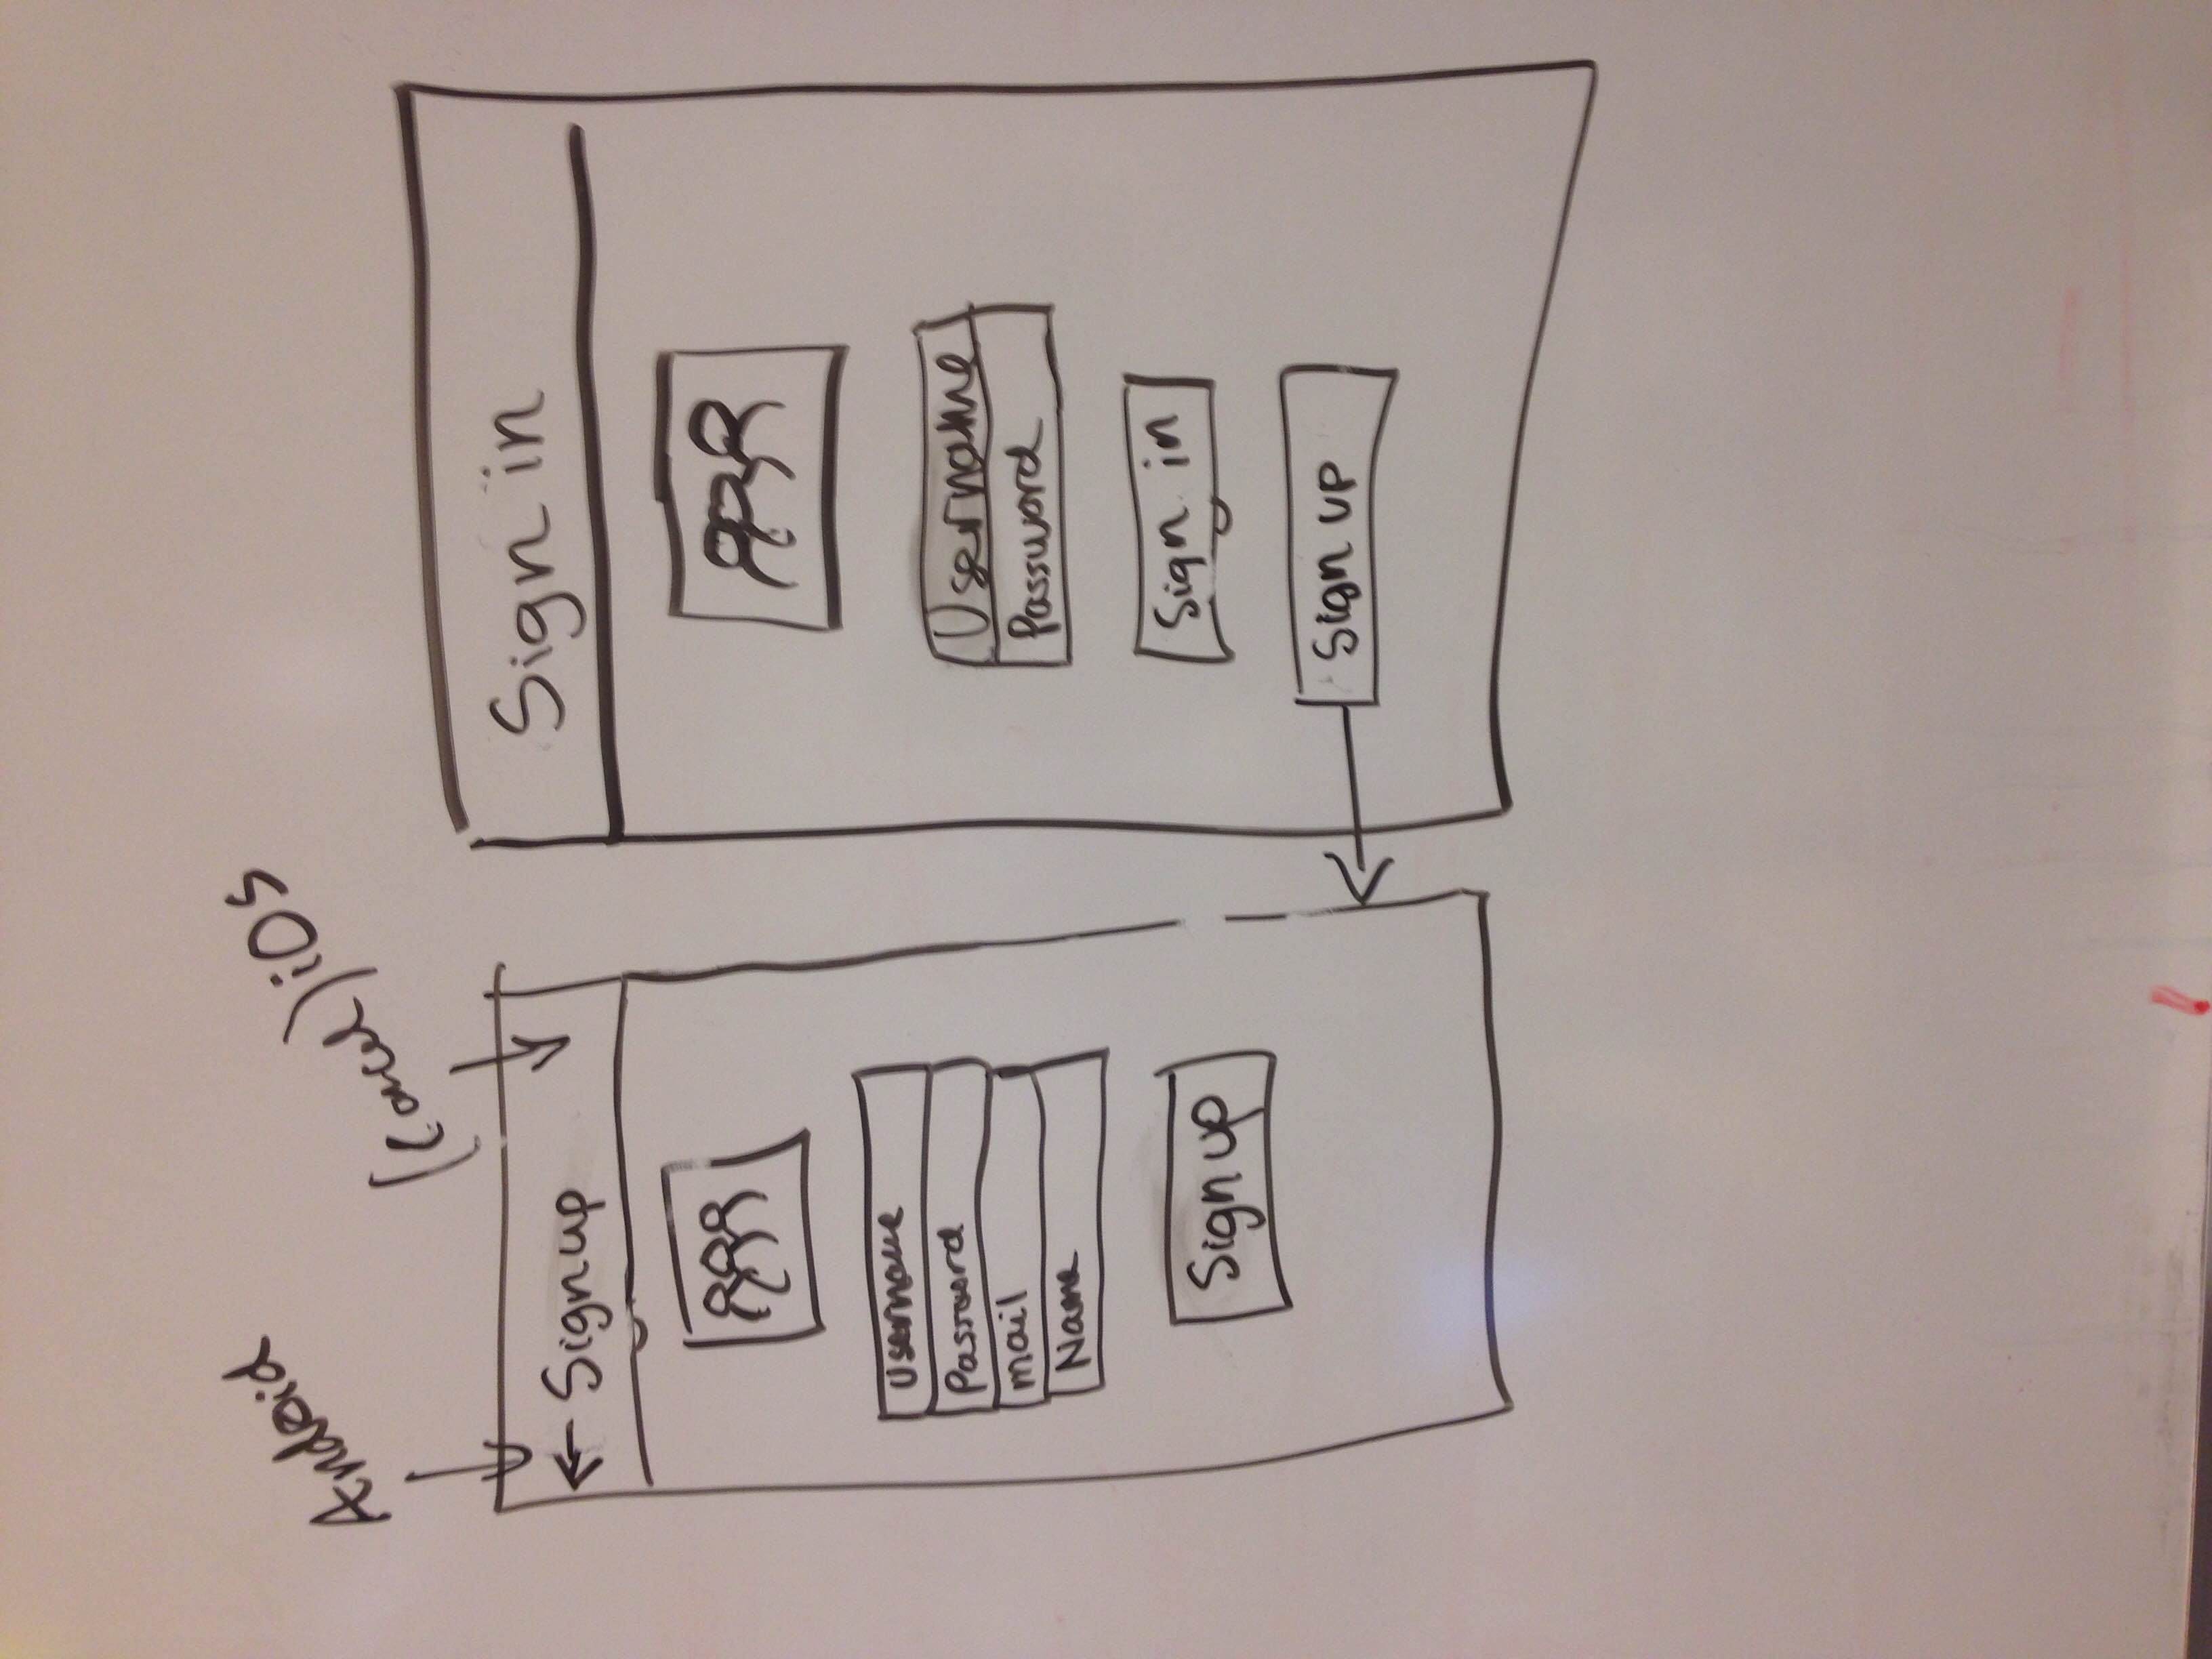
\includegraphics[height=7cm,angle=-90]{figs/v06/signin-whiteboard.jpg}
\caption{Design sketch from the planning phase}
\label{fig:design-sketch-6}
\end{figure}

\begin{figure}
\centering
\begin{subfigure}{.5\textwidth}
  \centering
  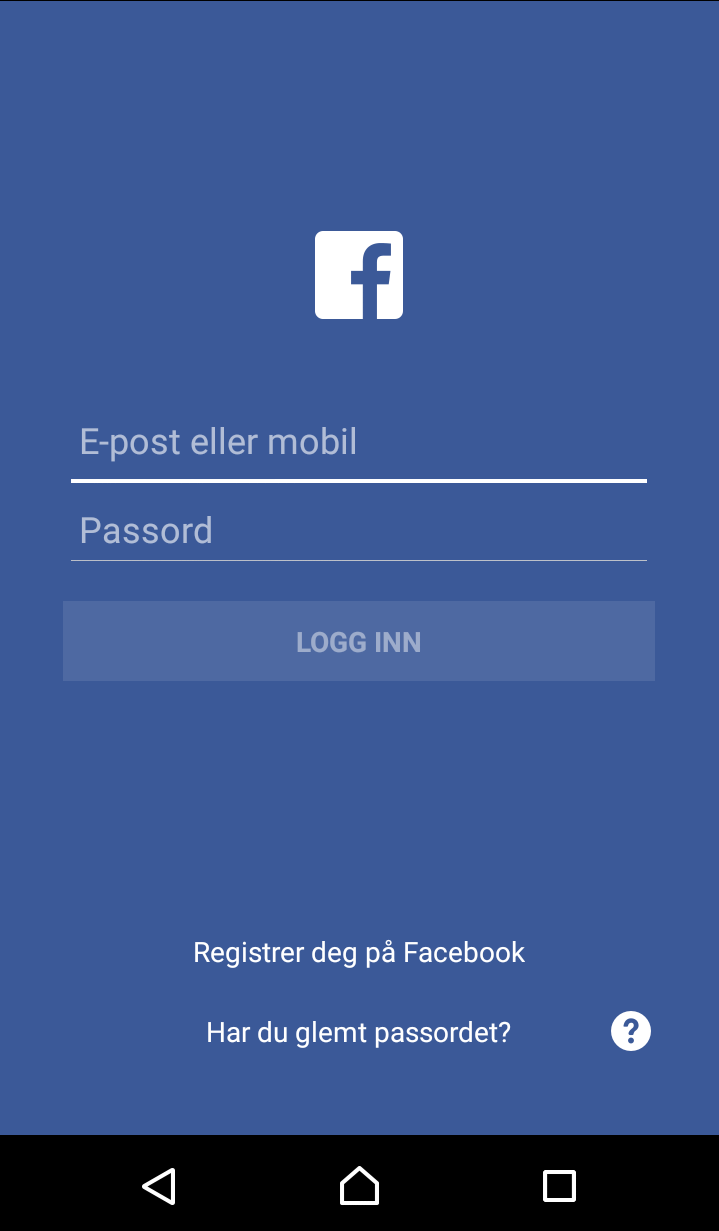
\includegraphics[width=.4\textwidth]{figs/v06/facebook-login-view-6.png}
  \caption{The Facebook login view}
  \label{fig:facebook-login-view-6}
\end{subfigure}%
\begin{subfigure}{.5\textwidth}
  \centering
  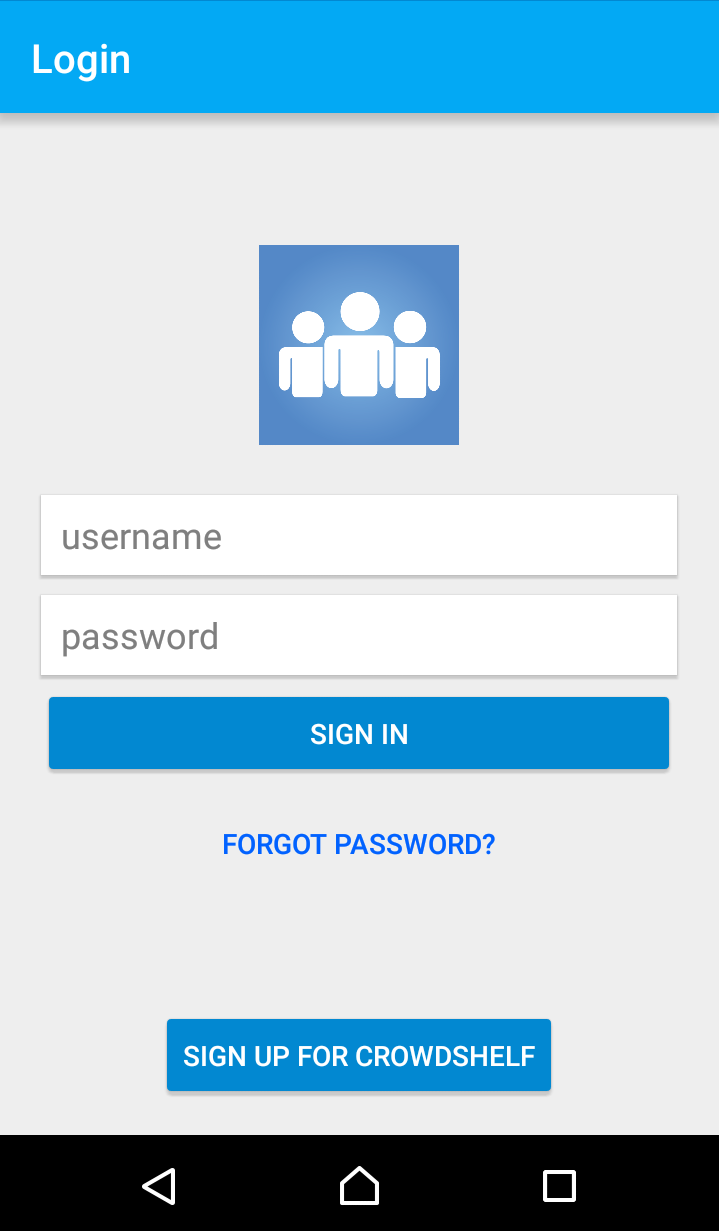
\includegraphics[width=.4\textwidth]{figs/v06/crowdshelf-login-view-6.png}
  \caption{The CrowdShelf sign in view}
  \label{fig:crowdshelf-login-view-6}
\end{subfigure}
\caption{Comparison of the Facebook login and CrowdShelf sign in design}
\label{fig:login-view-comparison-6}
\end{figure}


The customer representative also requested an email explaining the concept of the application, who the team were, and how to install the application, which he could send to his colleagues in Netlight to deploy the application.


\subsection{User stories}
\label{user-stories-v6}
These user stories were selected to describe the functionality of version 0.6.
\begin{enumerate}
    \item As a USER I want to be the only one who can edit My Shelf
    \item As a USER I want a secure authentication
\end{enumerate}

\subsection{Development}
This section describes what was developed during this version.

\subsubsection{Backend}
\label{v06-backend}
In this iteration the team wanted to finalize the \gls{backend} solution, and the results here is the result of both this iteration, and version 0.5. The reason for this was that the features had to be rolled out at once, as they were so tightly coupled. 

The iterations included complete user support, log-in and authorization. To be able to let user reset passwords and do similar operations, the team agreed that one would want the server to be able to send e-mails, so the iterations started by writing a general e-mail module within the server. The module provided a way to send an e-mail to send an e-mail to a list of addresses with a simple function call. The team then added templates for the different e-mails that had to be sent, and a helper-module that could handle building clean HTML- or text-documents, with user specific details. To accomplish this, the team used third party libraries. \cite{nodemailer}

When the e-mail service was ready, the team continued with updating the user model. This meant adding a password-field to the validation of user objects. The password had to be hashed, which was implemented with bcrypt. \cite{bcrypt} The login-request was also extended with a password-field, which was validated to be correct or not with the same bcrypt-library. If the login information was valid, the server was made to respond with the user object and a token. The token was generated with a library called Hat, and then added to a MonogDB-collection together with a expiration date 20 minutes ahead in time. \cite{hat} All requests that were not related to retrieving lost passwords, logging in or creating a new user now demanded a valid token. After 20 minutes the user had to login again. The login information could be saved locally in client application.

The team had a long discussion on how the authorization should be implemented. \gls{HTTPS}-certificates can be expensive, so it was not possible to use any real encryption. The team found that the token-strategy with a very limited time frame would be sufficient at this point, but that all connections should be encrypted if that could ever be a real option.

\subsubsection{Android}
\begin{description}
    \item[Features] \hfill\\
    \label{para:androidFeature06}
% Locally store token
The main focus for version 0.6 was authentication of the user in the application. This included only allowing changes to a user or a crowd if you have access to that specific user. This was implemented by demanding the user to enter both username and password when signing in. To be able to implement this feature the team also needed to add the possibility to create a user with a password. This was done by adding an extra text field to the create user screen, and including the user's input when sending data to the \gls{backend}. 

Since there is a possibility that the user can forget the password to their account. The team also implemented a feature for resetting a user's password. This was done by adding a new screen where a user could input a username. The \gls{backend} would then use this username to send an email to the user's email address. This email will contain a key the user needs to input into the application along with a new password. 

The last important feature for this version is that the team changed how the user uses the scanner. Before this version the user had to swipe or use the tabbed navigation bar at the top of the main screen to change to the scanner screen. In this version a new button was added at the top right of the screen. This button opened a new activity which used the camera of the device. This allowed the team to open the scanner from anywhere in the application. 

    \item[Structure] \hfill\\
Figure \ref{fig:AndroidStructure-06} shows the structure of the Android application after the features of version 0.6 was implemented. The most important activities for this version are the \code{ForgotPasswordAcitivty} activity which handles the resetting of a user's password and the \code{ScannerCaptureActivity} activity. The \code{ScannerCaptureActivity} activity is handling the scanning of barcode using the camera of the device and returning the barcode number to the \code{MainTabbedAcitivy} activity.

\begin{figure}
\centering
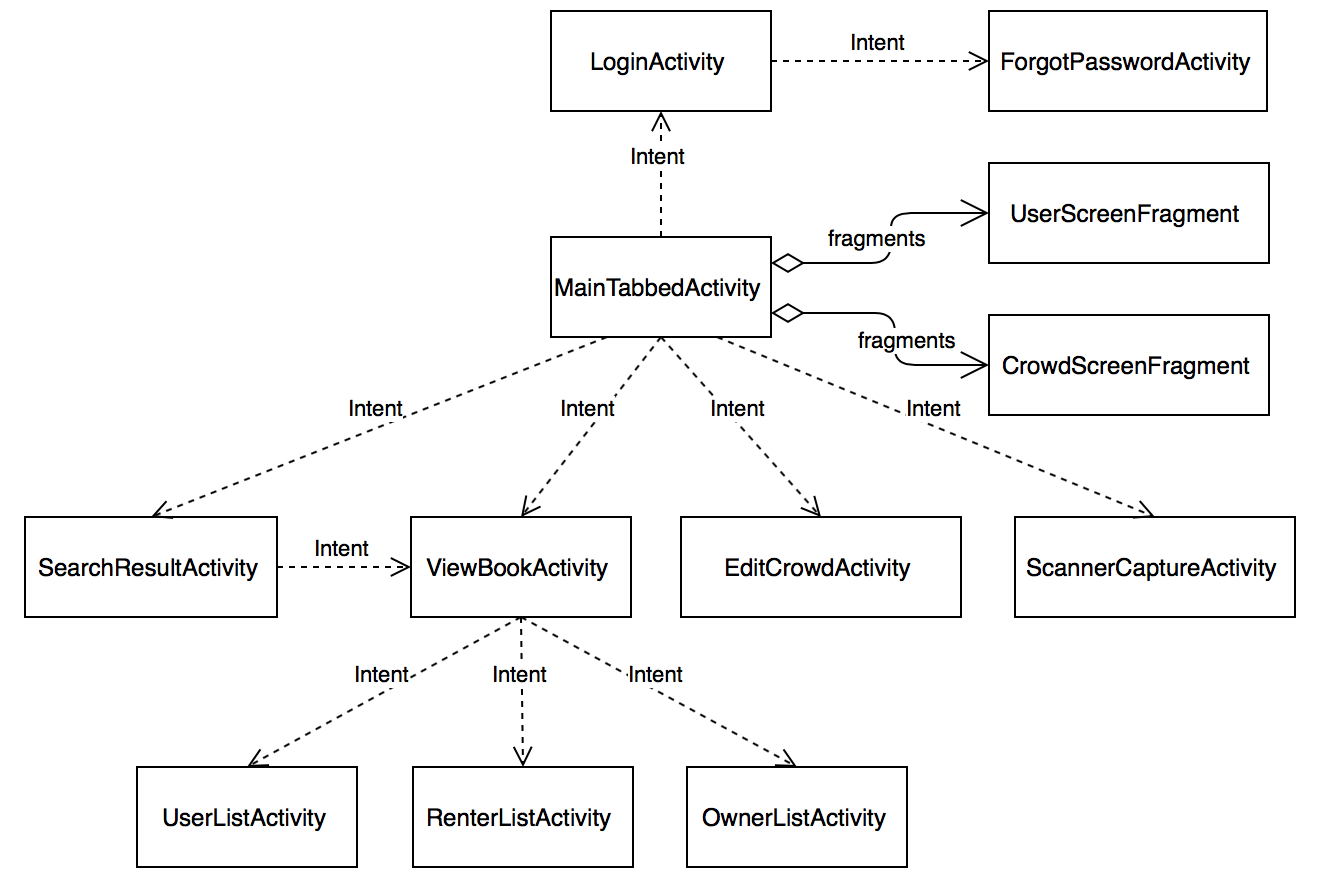
\includegraphics[width=\textwidth]{figs/v06/Android/AndroidStructure-06.png}
\caption{Android version 0.6 structure}
\label{fig:AndroidStructure-06}
\end{figure}

    \item[Design] \hfill\\
The main design change in version 0.6 is a result of the change in the scanner functionality. Because the scanner no longer is implemented in the application as a fragment it could no longer be a part of the tabs in the \code{MainTabbedActivity} activity. This is illustrated in figure \ref{fig:androidcompareDesign05}. Figure \ref{fig:androidcompareDesign06} shows how the scanner functionality is replaced in version 0.6. It is now a button in the top right of the screen opening a scanner view with the same functionality as in previous versions. Another design change that was made was to include a back button on some activities as a result of feedback from our users, this can be seen in figure \ref{fig:AndroidBackButton}

\begin{figure}
\centering
\begin{subfigure}{.5\textwidth}
  \centering
  
\includegraphics[width=.8\textwidth]{figs/v05/AndroidDesign-05.png}
  \caption{Version 0.5}
  \label{fig:androidcompareDesign05}
\end{subfigure}%
\begin{subfigure}{.5\textwidth}
  \centering
  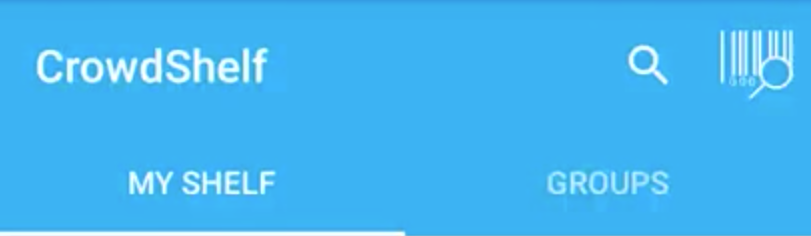
\includegraphics[width=.8\textwidth]{figs/v06/Android/AndroidDesign-06.png}
  \caption{Version 0.6}
  \label{fig:androidcompareDesign06}
\end{subfigure}
\caption{Android design changes from version 0.5 to version 0.6}
\label{fig:AndroidDesignComparison06}
\end{figure}

    \item[Bug fixes] \hfill\\
In version 0.5 the views for creating groups and editing existing groups used the same activity. This caused a bug that none of the buttons were hidden, which meant that buttons only relevant for existing groups were shown when creating a new group. If some of these buttons were clicked before the group was created it would result in an error. The solution to this bug was to make the buttons invisible if they were unusable for the current state of the view. 

Some minor bugs were also resolved. In previous versions it was not possible to create a group without any members. This functionality was desired when some users who tried to first create an empty group before later adding members.

As described in the Android feature paragraph the scanner as a fragment was removed from the \code{MainTabbedActivity} activity and rather used as an activity, the \code{ScannerCaptureActivity}. Previous to version 0.6 the application ran slow on some devices since the camera of the device were running continuously in the background. This was a result from having the scanner as a fragment. When changing the scanner feature to an activity it resulted in an improvement in the performance of the application.

\begin{figure}
\centering

\includegraphics[height=2cm]{figs/v06/backArrow.png}
\caption{The back arrow in action bar}
\label{fig:AndroidBackButton}
\end{figure}

\end{description}

\subsubsection{iOS}
\begin{description}
    \item[Features] \hfill\\
The new features in this version was a new register view, an updated login view, and user authentication. The new two views were meant to updated according to the design sketch, but there were not enough time to complete the task. To enable user authentication, the sign in procedure had to be updated in order to accept and store the new token received from the CrowdShelf \gls{backend}. This token had to be sent as a parameter in all requests to the server to verify that the user should have access to the data. This was fully implemented before the development ended, but a few issues with the server prevents the system from being fully operational.  

    \item[Design] \hfill\\
Apart from the uncompleted registration view, there were no major changes this version. The main difference was that the theme color was changed from Apple's default darker blue, to CrowdShelf's happier and lighter blue.


    \item[Feedback] \hfill\\
Due to the short time available for this version, the implementation was not completed, and therefore there is no feedback from usage of the applications or \gls{backend}. If there had been more time available, the clients and server would have been completed and distributed as a \gls{MVP} to Netlight. Then usage data could have been collected using Mixpanel in order to evaluate how the users adopt the new technology.

Unfortunately, there was not enough time to write the email to Netlight's employees either. This could have provided the users needed for the learning process.
\end{description}


\subsection{Version progress}
Because the \gls{backend} team had been working on user authentication during version 0.5, the velocity of the development on the clients was quite good. User authentication, email services and the updated login procedure was quickly added to the \gls{backend}, but a few bugs on both clients and the \gls{backend} caused the velocity to decrease. During the meeting with the customer representative \ref{app:customer-minutes-10} it was decided that the development should come to an end. Thus both applications were only partially functional and contained multiple bugs.

A blog post from the end of this version can be seen in figure \ref{fig:blog-week-11}. 

\begin{figure}
\centering
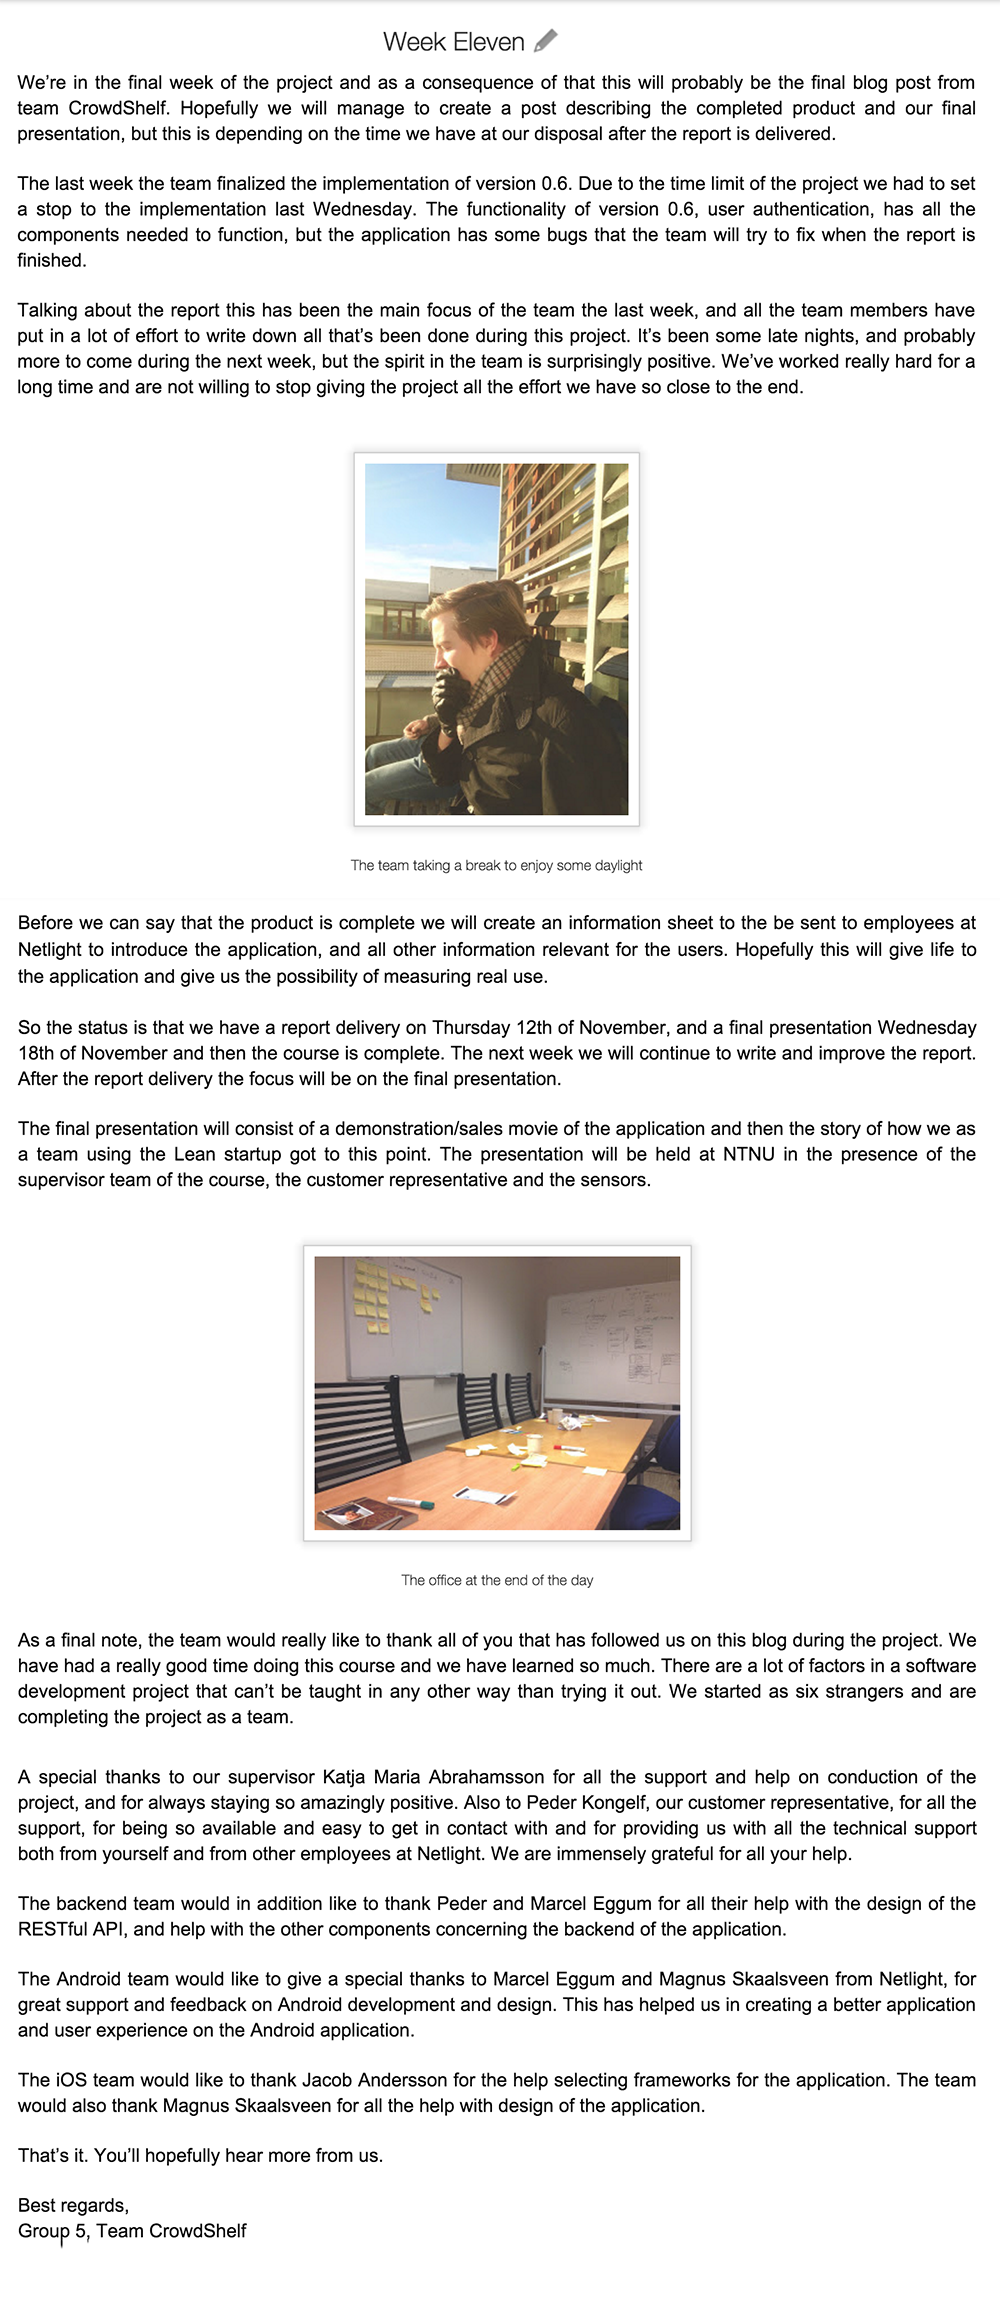
\includegraphics[height=\textheight]{figs/v06/week-11.png}
\caption{Blog post from week eleven}
\label{fig:blog-week-11}
\end{figure}

\subsection{Review}
After discussing with the customer representative it was decided that the implementation should be stopped to focus on the report. That decision made this the last version of the application. The result of this version which also is the final product of the application is concluded in the next section. 


\subsection{Summary}
As a summary of this version, the team started with the plan of implementing user authentication, and this feature was created. A consequence of the abrupt stop of implementation was that the last version contains many bugs. These bugs will be fixed after the report is delivered.

With version 0.6 complete the development part of the project is completed. Table \ref{version-schedule} lists all the versions completed with release dates and functionality included. Chapter \ref{chap:ArchitecturalDescription} includes a complete overview of the system architecture. A summary of the functionality in the applications and \gls{API} is described in section \ref{conclusion-system-overview}.

\begin{table}[]
\centering

\begin{tabular}{|L{3cm}|L{3cm}|L{8cm}|}
\hline
\textbf{Version} & \textbf{Release date} & \textbf{Description} \\
\hline
0.1 & 20/Sep/15 & This version produced two videos created to explain the product, and test the markets interest. \\
\hline
0.2 & 25/Sep/15 & A user has the possibility to view their books, scan the books barcode using the phones camera and add or remove those books. \\
\hline
0.3 & 07/Oct/15 & This version includes the feature of borrowing and returning books. The borrowed and lent out books are shown in the shelf view. \\
\hline
0.4 & 21/Oct/15 & This version includes group functionality, a way to find out what books users you know, or just want to share books with owns. \\
\hline
0.5 & 29/Oct/15 & In this version the possibility to search for books is included. A user can search globally of locally in their groups. \\
\hline
0.6 & 06/Nov/15 & This version has updated the login functionality by adding user validation.\\
\hline
\end{tabular}
\caption{Schedule of versions}
\label{version-schedule}
\end{table}